\chapter{Resultados}      \label{Resultados}

No Capítulo anterior, foi visto o procedimento metodológico de otimização e modelagem inversa por aprendizagem profunda. Neste Capítulo, são mostrados os resultados do procedimento para os dispositivos estudados. Na Seção \ref{Resultado Circulador}, são mostrados os resultados referentes aos dois circuladores baseados em cristais fotônicos.



\section{Circulador}      \label{Resultado Circulador}

Os resultados da modelagem inversa dos dois circuladores de junção-T baseados em cristal fotônico estão apresentados nesta Seção. A Fig. \ref{fig: DipoleOptimization} mostra a resposta em frequência do circulador de ressonância \textit{dipolo} após o procedimento de otimização proposto neste trabalho.

\begin{figure}[H]
	\centering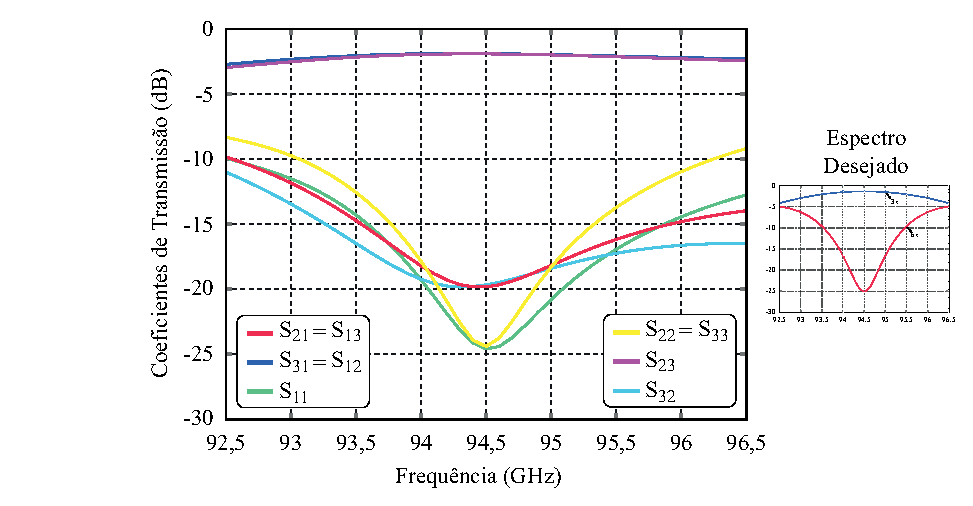
\includegraphics{04-Figuras/DipoleOptimization.eps}
	\caption{Resposta em frequência do circulador dipolo após a modelagem inversa.}
    Fonte: do Autor.
	\label{fig: DipoleOptimization}
\end{figure}

Nota-se que o procedimento de modelagem inversa foi satisfatório e é possível notar a proximidade com a resposta em frequência desejada (ver Fig. \ref{fig: PhcTargetFrequencyResponse} para mais detalhes). O resultado do circulador com ressonância \textit{quadrupolo} também apresenta êxito na aproximação com a resposta em frequência desejada, como mostra a Fig. \ref{fig: QuadrupoleOptimization}.

\begin{figure}[H]
	\centering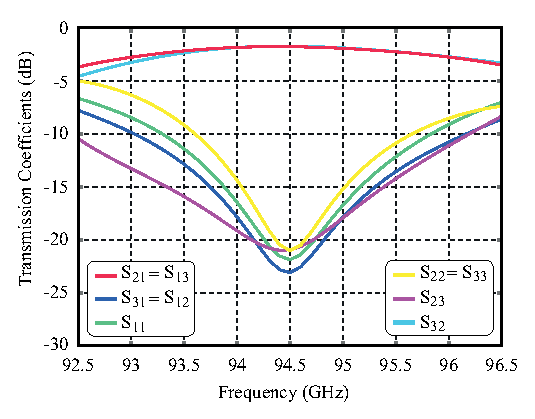
\includegraphics{04-Figuras/QuadrupoleOptimization.eps}
	\caption{Resposta em frequência do circulador quadrupolo após a modelagem inversa.}
    Fonte: do Autor.
	\label{fig: QuadrupoleOptimization}
\end{figure}

A geometria final de ambos circuladores está mostrada na Fig. \ref{fig: PhCGeometryOptimization}. Cada variável geométrica otimizada está abordada detalhadamente na Seção \ref{PhC} do Apêndice \ref{Apendice}.

\begin{figure}[H]
    \centering
    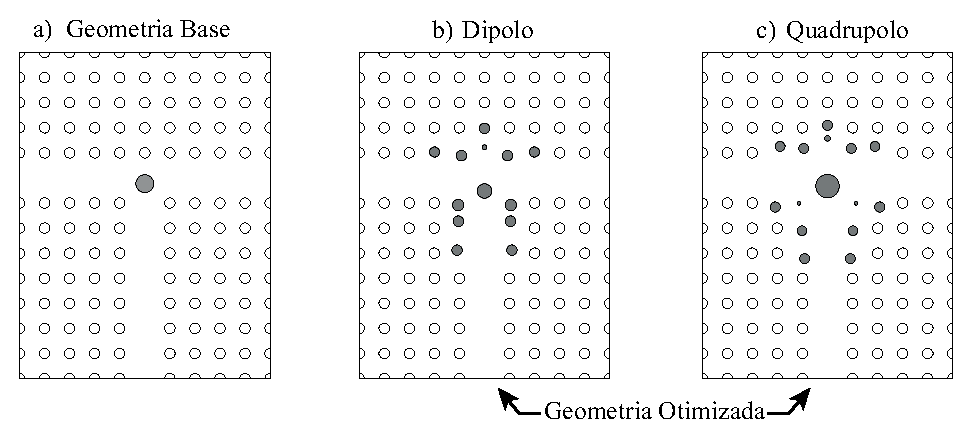
\includegraphics{04-Figuras/PhCGeometryOptimization.eps}
    \caption{Geometria dos circuladores após a otimização. a) Geometria base. b) Geometria final do circulador dipolo. c) Geometria final do circulador quadrupolo.} \par
    Fonte: do Autor.
    \label{fig: PhCGeometryOptimization}
\end{figure}

A Tabela \ref{tab: MSECirculador} mostra que para o circulador dipolo foram necessários $641$ \textit{Loops} para o algoritmo chegar na resposta em frequência mostrada na Fig. \ref{fig: DipoleOptimization}. Para o circulador quadrupolo, foram $1487$ \textit{Loops} até o algorítimo atingir a resposta em frequência mostrada na Fig. \ref{fig: QuadrupoleOptimization}.





\begin{table}[H]
    \centering
    \caption{Comparação do desempenho de otimização dos divisores.}
\begin{tabular}{ccc}
\hline
Dispositivo           & Loop & MSE    \\ \hline
Circulador Dipolo     & 641  & 0,0059 \\
Circulador Quadrupolo & 1487 & 0,0083 \\ \hline
\end{tabular}

    \label{tab: MSECirculador}

    \vspace{2.5mm}
    Fonte: do Autor.

\end{table}

A Fig. \ref{fig: MSEDipole} mostra a evolução da função custo à medida que o processo exemplificado na Fig. \ref{fig: OptimizationAlgorithm} é executado, de forma que o banco de dados do circulador dipolo incrementa até atingir $641$ \textit{Loops}. Nesse estágio, a resposta em frequência do dispositivo foi aproximada do espectro desejado, conforme o algoritmo mostrado na Fig. \ref{fig: OptimizationAlgorithm}.

\begin{figure}[H]
	\centering\includegraphics{04-Figuras/MSEDipole.eps}
	\caption{Evolução da função custo para o circulador dipolo.}
    Fonte: do Autor.
	\label{fig: MSEDipole}
\end{figure}

O mesmo comportamento foi observado no gráfico da avaliação da função custo para o circulador de ressonância quadrupolo, como mostra a Fig. \ref{fig: MSEQuadrupole}, à medida que o banco de dados do referido circulador incrementa até atingir $1487$ \textit{Loops}.

\begin{figure}[H]
	\centering\includegraphics{04-Figuras/MSEQuadrupole.eps}
	\caption{Evolução da função custo para o circulador quadrupolo.}
    Fonte: do Autor.
	\label{fig: MSEQuadrupole}
\end{figure}

A avaliação da função custo mostrada nas Figs. \ref{fig: MSEDipole} e \ref{fig: MSEQuadrupole}, são referentes ao desempenho da rede neural em relação ao banco de dados de teste, particionado em 10\% (ver Seção \ref{PhC} do Apêndice \ref{Apendice}). Nesse sentido, quanto mais informações (dados) a rede neural tem sobre o ambiente (dispositivos estudados), maior é a sua acurácia (portanto, menor o erro) em predizer a geometria dos dispositivos.

\newpage
\subsection{Fatores de Qualidade}

Cada curva $S_{ij}$ da resposta em frequência foi avaliada através de métricas de desempenho. Desta maneira, foi possível avaliar o erro associado (MSE) entre os valores de desempenho considerados ótimos (valor ideal) e os valores obtidos no processo de otimização por aprendizagem profunda (valor otimizado).

A Tabela \ref{tab: FQ_Dipolo} mostra os fatores de qualidade para o circulador de ressonância dipolo. 





\begin{table}[H]
    \centering
    \caption{Fatores de qualidade avaliados para o circulador de ressonância dipolo.}
    \begin{tabular}{cccc}
\hline
Fatores          & Valor Ideal            & Valor Otimizado & \multicolumn{1}{l}{Erro Associado (MSE)} \\ \hline
$\Delta F_{11}$  & 94,5 GHz               & 94,5 GHz        & 0                                        \\
$\Delta F_{21}$  & 94,5 GHz               & 94,5 GHz        & 0                                        \\
$\Delta F_{31}$  & 94,5 GHz               & 94,5 GHz        & 0                                        \\
$\Delta F_{12}$  & 94,5 GHz               & 94,5 GHz        & 0                                        \\
$\Delta F_{22}$  & 94,5 GHz               & 94,5 GHz        & 0                                        \\
$\Delta F_{32}$  & 94,5 GHz               & 94,3 GHz        & 0,04                                     \\
$\Delta F_{13}$  & 94,5 GHz               & 94,4 GHz        & 0,01                                     \\
$\Delta F_{23}$  & 94,5 GHz               & 94,5 GHz        & 0                                        \\
$\Delta F_{33}$  & 94,5 GHz               & 94,5 GHz        & 0                                        \\
$\Delta T1_{13}$ & -1 dB                  & -1,7 dB         & 0,49                                     \\
$\Delta T1_{31}$ & -1 dB                  & -1,7 dB         & 0,49                                     \\
$\Delta T1_{12}$ & -1 dB                  & -1,7 dB         & 0,49                                     \\
$\Delta T2_{11}$ & $\leq \textrm{-20 dB}$ & -24,9 dB        & 0                                        \\
$\Delta T2_{21}$ & $\leq \textrm{-20 dB}$ & -19,98 dB       & 0,04                                     \\
$\Delta T2_{22}$ & $\leq \textrm{-20 dB}$ & -24,85 dB       & 0                                        \\
$\Delta T2_{32}$ & $\leq \textrm{-20 dB}$ & -20,1 dB        & 0                                        \\
$\Delta T2_{13}$ & $\leq \textrm{-20 dB}$ & -20,1 dB        & 0                                        \\
$\Delta T2_{33}$ & $\leq \textrm{-20 dB}$ & -24,85 dB       & 0                                        \\
$BW$             & - -                    & 1,5 GHz         & - -                                      \\ \hline
\end{tabular}

    \label{tab: FQ_Dipolo}

    \vspace{2.5mm}
    Fonte: do Autor.

    \end{table}

Assim, $\Delta F_{ij}$ mostra a ressonância de cada curva em relação à frequência central de operação ($F_{c} = $ 94,5 GHz). A maior parte das curvas foram otimizadas (erro igual a zero), com excessão das curvas $\Delta F_{32}$ e $\Delta F_{13}$, com erros de 0,04 e 0,01, respectivamente. As curvas $\Delta T1_{ij}$ têm por objetivo de otimização serem maximizadas a $\textrm{-1 dB}$, e em todos os casos houve um erro de 0,49 em relação ao ao valor obtido de $\textrm{-1,7 dB}$. Para as curvas $\Delta T2_{ij}$, apenas $\Delta T2_{21}$ obteve erro diferente de zero (0,04), enquanto que as demais foram otimizadas para um valor abaixo de $\textrm{-20 dB}$.

Para o circulador de ressonância quadrupolo, os fatores de qualidade estão mostrados na Tabela \ref{tab: FQ_Quadrupolo}.





\begin{table}[H]
    \centering
    \caption{Fatores de qualidade avaliados para o circulador de ressonância quadrupolo.}
    \begin{tabular}{cccc}
\hline
Fatores          & Valor Ideal            & Valor Otimizado & \multicolumn{1}{l}{Erro Associado (MSE)} \\ \hline
$\Delta F_{11}$  & 94,5 GHz               & 94,5 GHz        & 0                                        \\
$\Delta F_{21}$  & 94,5 GHz               & 94,4 GHz        & 0,01                                     \\
$\Delta F_{31}$  & 94,5 GHz               & 94,5 GHz        & 0                                        \\
$\Delta F_{12}$  & 94,5 GHz               & 94,5 GHz        & 0                                        \\
$\Delta F_{22}$  & 94,5 GHz               & 94,5 GHz        & 0                                        \\
$\Delta F_{32}$  & 94,5 GHz               & 94,4 GHz        & 0,01                                     \\
$\Delta F_{13}$  & 94,5 GHz               & 94,4 GHz        & 0,01                                     \\
$\Delta F_{23}$  & 94,5 GHz               & 94,4 GHz        & 0,01                                     \\
$\Delta F_{33}$  & 94,5 GHz               & 94,5 GHz        & 0                                        \\
$\Delta T1_{21}$ & -1 dB                  & -1,76 dB        & 0,57                                     \\
$\Delta T1_{32}$ & -1 dB                  & -1,72 dB        & 0,51                                     \\
$\Delta T1_{13}$ & -1 dB                  & -1,76 dB        & 0,57                                     \\
$\Delta T2_{11}$ & $\leq \textrm{-20 dB}$ & -21,87 dB       & 0                                        \\
$\Delta T2_{31}$ & $\leq \textrm{-20 dB}$ & -23,09 dB       & 0                                        \\
$\Delta T2_{12}$ & $\leq \textrm{-20 dB}$ & -23,09 dB       & 0                                        \\
$\Delta T2_{22}$ & $\leq \textrm{-20 dB}$ & -20,97 dB       & 0                                        \\
$\Delta T2_{23}$ & $\leq \textrm{-20 dB}$ & -20,99 dB       & 0                                        \\
$\Delta T2_{33}$ & $\leq \textrm{-20 dB}$ & -21,02 dB       & 0                                        \\
$BW$             & - -                    & 0,9 GHz         & - -                                      \\ \hline
\end{tabular}

    \label{tab: FQ_Quadrupolo}

    \vspace{2.5mm}
    Fonte: do Autor.

    \end{table}

A otimização das curvas $\Delta F_{ij}$ para a frequência central ($\textrm{94,5 GHz}$) obteve erro de 0,01 para as curvas $\Delta F_{21}$, $\Delta F_{32}$, $\Delta F_{13}$ e $\Delta F_{23}$. As curvas $\Delta T1_{ij}$ obtiveram erro de 0,57 para as curvas $\Delta T1_{21}$ e $\Delta T1_{13}$ e de 0,51, para a curva $\Delta T1_{32}$. Todas as curvas $\Delta T2_{ij}$ cumpriram o objetivo de otimização para serem minimizadas abaixo de $\textrm{-20 dB}$.

De forma geral, nas Tabelas \ref{tab: FQ_Dipolo} e \ref{tab: FQ_Quadrupolo}, há parâmetros referentes a $\Delta T2_{ij}$ que têm erro associado igual a \textit{zero}, pois cumpriram a condição $\leq \textrm{-20 dB}$ (não importando o quão menor $\Delta T2_{ij}$ for de $\textrm{-20 dB}$). Neste caso, o erro (MSE) será diferente de zero nas situações em que $\Delta T2_{ij}$ for maior que $\textrm{-20 dB}$.

A largura de banda $BW$ foi calculada considerando os pontos $f_{1}$ e $f_{2}$ (ver Fig. \ref{fig: QualityFactor}) das curvas mais internas a $\textrm{-15 dB}$.